\documentclass[dvipsnames,12pt]{book}
\usepackage{tikz}

\graphicspath{{Images/}}

%Hey, if you're using this preamble it means that it was probably written by Stefano Graziosi (me). If you see something that doesn't make sense, feel free to email me at stefano.graziosi@studbocconi.it
%p.s. in case it's not already evident from the preamble, I'm not a professional LaTeX user, so I'm sure there are better ways to do things. I'm just trying to make it work.

%------------------------------------------------------------------------------
%           LAST UPDATE: 30-01-2025
%------------------------------------------------------------------------------

%I don't own copyright on anything, I just literally copied and pasted together a bunch of stuff.

%Credit goes to the original authors.

%------------------------------------------------------------------------------
%           Packages
%------------------------------------------------------------------------------

\usepackage{fancyhdr}
\usepackage[dvipsnames]{xcolor}
\usepackage[many]{tcolorbox}
\usepackage[all]{xy}
\usepackage{tcolorbox}
\usepackage{graphicx}
\usepackage{hyperref}
\usepackage{xcolor}    
\usepackage{wrapfig}
\usepackage{amsmath, amssymb, amsthm}
\usepackage{titlesec}
\usepackage{halloweenmath}
\usepackage{enumitem}
\usepackage{listings}

\usepackage[T1]{fontenc}                            % Font Styling
\usepackage{lmodern,mathrsfs}


\usepackage{mathtools,amsthm,amssymb,amsfonts,bm}   % Math Presets
\usepackage{thmtools,amsmath}
\usepackage{array,tabularx,booktabs}                % Table Presets
\usepackage{graphicx,wrapfig,float,caption}         % Figure Presets
\usepackage{setspace,multicol}                      % Text Presets
\usepackage{tikz,physics}                           % Physics Presets

\usepackage{titlepic}
\usepackage{pdfpages}

%------------------------------------------------------------------------------
%           Geometry
%------------------------------------------------------------------------------

\usepackage[a4paper,margin=1in]{geometry}
%\usepackage[margin=1in]{geometry}

\renewcommand{\chaptername}{Lecture}
%\renewcommand\thesection{P~\arabic{section}}

%------------------------------------------------------------------------------
%           Colours
%------------------------------------------------------------------------------

\definecolor{sgblue}{rgb}{0, 169, 211}
\definecolor{sggreen}{rgb}{0, 164, 0}
\definecolor{sgpurple}{rgb}{99, 0, 165}
\definecolor{sgyellow}{rgb}{255, 211, 0}
\definecolor{sgorange}{rgb}{255, 127, 20}

\definecolor{sbblue}{rgb}{219, 248, 254}
\definecolor{sbgreen}{rgb}{223, 255, 218}
\definecolor{sbpurple}{rgb}{241, 220, 255}

\definecolor{codegreen}{rgb}{0,0.6,0}
\definecolor{codegray}{rgb}{0.5,0.5,0.5}
\definecolor{codepurple}{rgb}{0.58,0,0.82}
\definecolor{backcolour}{rgb}{0.95,0.95,0.92}

%------------------------------------------------------------------------------
%           Environments
%------------------------------------------------------------------------------

%Standard \latex box

\newtcolorbox{mybox}[3][]
{
  colframe = #2!25,
  colback  = #2!10,
  coltitle = #2!20!black,  
  title    = {#3},
  #1,
}

%Standard "Problem" environment

\newtheorem{problem}{Problem}

%Personalised "Solution" environment

\newenvironment{solution}[1][\it{\textcolor{MidnightBlue}{Solution}}]{\textbf{#1. } }{\textcolor{MidnightBlue}{$\square$}}


% ----------------------------------------------------------------------
%           Special Environments 
% ----------------------------------------------------------------------

\newlength{\spacelength}
\settowidth{\spacelength}{\normalfont\ }
\declaretheoremstyle[
    headfont={\bfseries\sffamily\footnotesize},
    notefont={\normalfont},
    bodyfont={\normalfont},
    headpunct={\relax},%\newline,
    headformat={%
        \makebox[0pt][r]{\NAME\ \NUMBER\hspace{\marginparsep}}\hskip-\spacelength{\normalsize\NOTE}},
]{theorem}

\tcolorboxenvironment{theorem}{
  boxrule=0pt,
  boxsep=0pt,
  colback={White},
  enhanced jigsaw, 
  borderline west={1pt}{0pt}{ForestGreen},
  sharp corners,
  before skip=10pt,
  after skip=10pt,
  left=5pt,
  right=5pt,
  breakable,
}

\declaretheorem[style=theorem]{proposition}

\let\proof\relax
\let\endproof\relax

\declaretheoremstyle[
    headfont={\bfseries\sffamily\footnotesize},
    notefont={\normalfont},
    bodyfont={\normalfont},
    headpunct={\relax},%\newline,
    headformat={%
        \makebox[0pt][r]{\NAME\ \NUMBER\hspace{\marginparsep}}\hskip-\spacelength{\normalsize\NOTE}},
]{theorem}

\tcolorboxenvironment{proposition}{
  boxrule=0pt,
  boxsep=0pt,
  colback={White},
  enhanced jigsaw, 
  borderline west={1pt}{0pt}{Mulberry},
  sharp corners,
  before skip=10pt,
  after skip=10pt,
  left=5pt,
  right=5pt,
  breakable,
}

\declaretheorem[style=theorem]{theorem}

\let\proof\relax
\let\endproof\relax

\declaretheoremstyle[
    headfont={\small\scshape},
    notefont={\normalfont},
    bodyfont={\normalfont},
    headpunct={\relax},
    headformat={%
        \makebox[0pt][r]{\NAME\hspace{\marginparsep}}\hskip-\spacelength{\NOTE}},
]{proof}

\tcolorboxenvironment{proof}{
  boxrule=0pt,
  boxsep=0pt,
  blanker,
  borderline west={1pt}{0pt}{black},
  before skip=10pt,
  after skip=10pt,
  left=5pt,
  right=5pt,
  breakable,
}

\declaretheoremstyle[
    headfont={\footnotesize\itshape},
    notefont={\normalfont},
    bodyfont={\normalfont},
    headpunct={\relax},
    headformat={%
        \makebox[0pt][r]{\NAME\hspace{\marginparsep}}\hskip-\spacelength{\NOTE}},
]{claim}

\declaretheorem[
    style=proof,
    qed=\qedsymbol]{proof}

\declaretheorem[style=claim]{Intuition}

\theoremstyle{theorem}
\newtheorem{ques}{Question}

\theoremstyle{theorem}
\newtheorem{definition}{Definition}
\tcolorboxenvironment{definition}{
  boxrule=0pt,
  boxsep=0pt,
  colback={White},
  enhanced jigsaw, 
  borderline west={1pt}{0pt}{Cerulean},
  sharp corners,
  before skip=10pt,
  after skip=10pt,
  left=5pt,
  right=5pt,
  breakable,
}

\theoremstyle{theorem}
\newtheorem{lemma}{Lemma}
\tcolorboxenvironment{lemma}{
  boxrule=0pt,
  boxsep=0pt,
  blanker,
  borderline west={1pt}{0pt}{Rhodamine},
  before skip=10pt,
  after skip=10pt,
  sharp corners,
  left=5pt,
  right=5pt,
  breakable,
}

\theoremstyle{theorem}
\newtheorem{remark}{Remark}
\tcolorboxenvironment{remark}{
  boxrule=0pt,
  boxsep=0pt,
  colback={White},
  enhanced jigsaw, 
  borderline west={1pt}{0pt}{BurntOrange},
  before skip=10pt,
  after skip=10pt,
  sharp corners,
  left=5pt,
  right=5pt,
  breakable,
}

\theoremstyle{theorem}
\newtheorem{corollary}{Corollary}
\tcolorboxenvironment{corollary}{
  boxrule=0pt,
  boxsep=0pt,
%  colback={White!100!WildStrawberry},
  enhanced jigsaw,
  borderline west={1pt}{0pt}{WildStrawberry},
  before skip=10pt,
  after skip=10pt,
  sharp corners,
  left=5pt,
  right=5pt,
  breakable,
}

\theoremstyle{theorem}
\newtheorem{example}{Example}
\tcolorboxenvironment{example}{
  boxrule=0pt,
  boxsep=0pt,
  blanker,
  borderline west={1pt}{0pt}{Dandelion},
  before skip=10pt,
  after skip=10pt,
  sharp corners,
  left=5pt,
  right=5pt,
  breakable,
}


\theoremstyle{claim}
\newtheorem{intu}{Intuition}

\theoremstyle{claim}
\newtheorem{solu}{Solution}

%------------------------------------------------------------------------------
%           Code Listing Environment
%------------------------------------------------------------------------------

\lstdefinestyle{mystyle}{
    backgroundcolor=\color{backcolour},   
    commentstyle=\color{codegreen},
    keywordstyle=\color{magenta},
    numberstyle=\tiny\color{codegray},
    stringstyle=\color{codepurple},
    basicstyle=\ttfamily\footnotesize,
    breakatwhitespace=false,         
    breaklines=true,                 
    captionpos=b,                    
    keepspaces=true,                 
    numbers=left,                    
    numbersep=5pt,                  
    showspaces=false,                
    showstringspaces=false,
    showtabs=false,                  
    tabsize=2
}

\lstset{style=mystyle}

\titlepic{
    \makebox[0pt][c]{\hspace*{0.135cm}%
    
\includegraphics[width=\paperwidth]{20888 Logo.png}
    }
}
\title{20888 Foundations of Social Sciences - Module 2A \\[0.2cm] {\Large \textit{Institutions, Government and Society}} \\[1cm] \textbf{Lecture Notes}}
\author{Stefano Graziosi, Università Bocconi}
\date{\today}

\begin{document}

\maketitle

\tableofcontents

\part{History of Economic Thought}

    \chapter[Exchange and Political Community]{Aristotle \\[0.6cm] \textit{Exchange and Political Community}}

            \section{Politics - Book I}

        \subsection{Introduction: The Polis and the Oikos}

            One of Aristotle’s key distinctions in Politics Book I is between the \textit{polis} (the city or political community) and the \textit{oikos} (the household or family). For the ancient Greeks, these two spheres represented fundamentally different realms of human activity:
    
                \begin{definition}[oikos]
                    The \textit{oikos} is the sphere of necessity—it deals with survival, daily needs, and household management.
                \end{definition}
    
                \begin{definition}[polis]
                    The \textit{polis} is the sphere of freedom—it aims at enabling people to live the good life, one marked by virtuous activity and flourishing.
                \end{definition}

            \subsubsection{A Central Question}

                \begin{quote}
                    Should the state be managed as an enterprise or not? Should an entrepreneur manage the state as if it were his enterprise?
                \end{quote}

                This question highlights a tension still relevant today: can (or should) the principles of economic management (focused on profit, efficiency, resource allocation) govern the political realm (focused on justice, common good, and the flourishing of citizens)?
                
                Aristotle’s answer—developed throughout his Politics—is that the methods of running a household economy (oikos) and the methods of running a political community (polis) are necessarily different. Politics, for Aristotle, is not merely a larger-scale version of household management.
\newpage
            \subsection{Digression: Hannah Arendt}

                Hannah Arendt (1906–1975) was a 20th-century political theorist whose works often draw on ancient Greek thought. Two of her major works are:
\vspace{-0.05cm}
                    \begin{itemize}
                        \item \textit{The Origins of Totalitarianism} (1951) – An analysis of totalitarian regimes (Nazi Germany, Stalinist Russia), focusing on how they subverted the public realm and destroyed the capacity for genuine political action.
                        \item \textit{The Human Condition} (1958) – An exploration of what it means to be human in the modern age, distinguishing different kinds of human activities (labor, work, and action) and reflecting on the modern eclipse of authentic political life.
                    \end{itemize}

                \subsubsection{Arendt on “Political Economy”}

                    Arendt famously claimed that the term “\textbf{political economy}” is an \textit{oxymoron}. \textbf{Why?} In antiquity, politics and economics were understood to be distinct spheres:
                            \begin{itemize}
                                \item \textbf{Economics} (oikonomia) is the management of the household (oikos), governed by necessity and the administration of resources.
                                \item \textbf{Politics} (the life of the polis) is the realm of public freedom, speech, and action, dedicated to matters of justice and the common good.
                            \end{itemize}

                    For Arendt, and following Aristotle, conflating these two realms—treating the political community as though it should be run by the same principles as a household or enterprise—distorts the essence of politics, which involves deliberation about the just and the unjust, the good and the bad, and the shared life of citizens.
\vspace{-0.25cm}
                \subsubsection{Arendt’s Three Human Activities}

                    In \textit{The Human Condition}, Arendt distinguishes three fundamental human activities:
\vspace{-0.05cm}
                        \begin{enumerate}
                            \item \textbf{Animal laborans} (the laboring animal)
                                \begin{itemize}
                                    \item Concerned with biological life (eating, sleeping, reproducing).
                                    \item Its tasks are repetitive and cyclical, tied to necessity.
                                \end{itemize}
                            \item \textbf{Homo faber} (the maker or builder)
                                \begin{itemize}
                                    \item Concerned with production or fabrication—crafting things that endure beyond their maker’s lifespan (e.g., art, tools, buildings).
                                    \item Gives the world a degree of permanence and durability.
                                \end{itemize}
                            \item \textbf{Zoon politikon} (the political animal)
                                \begin{itemize}
                                    \item Concerned with action (praxis) and speech, particularly in the public realm.
                                    \item Seeks the good life through debate, deliberation, and collective decision-making, embodying the classic Greek notion of full human flourishing.
                                \end{itemize}
                        \end{enumerate}

                    \begin{remark}
                        In ancient Greece, these spheres were more distinctly separated. Today, modern societies often conflate or subordinate the political (the realm of freedom and debate) to the economic (the realm of necessity and consumption)
                    \end{remark}

                \subsection{Succession and Priority}

                    \begin{remark}[Succession]
                        \textit{oikos} \(\rightarrow\) \textit{kòme} \(\rightarrow\) \textit{polis}
                    \end{remark}
            
                    Aristotle observes a developmental sequence in human communities: from the family (\textit{oikos}), to the village (\textit{kòme}), and finally to the city-state (\textit{polis}). However, he also asserts that the polis is by nature prior to the household and the individual (a statement he elaborates on in Politics 1253a).

                    While it might seem that the household comes “first,” Aristotle’s point is that the fully realized form of human association—the polis—logically and ontologically precedes the household in importance: only within a polis can human beings achieve the higher ends of justice and virtue.
            

        \section{Zoon Politikon}

            In Book I of the Politics, Aristotle famously argues that human beings are political animals (zoon politikon) more so than any other gregarious or social creatures. Unlike bees or ants, which also cooperate, humans have a unique capacity for logos—reasoned speech. This capacity allows us to discuss justice, goodness, advantageous vs. harmful, and other moral distinctions in ways that mere instinctual signalling cannot.

            \begin{quote}
                It is thus clear that man is a political animal (zoon politikon), in a higher degree than bees or other gregarious animals. Nature, according to our theory, makes nothing in vain; and man alone of the animals is furnished with the faculty of language. 
                
                The mere making of sounds serves to indicate pleasure and pain, and is thus a faculty that belongs to animals in general: their nature enables them to attain the point at which they have perceptions of pleasure and pain, and can signify those perceptions to one another.

                But language serves to declare what is advantageous and what is the reverse, and it is the peculiarity of man, in comparison with other animals, that he alone possesses a perception of good and evil, of the just and the unjust, and other similar qualities; and it is association in these things which makes a family (oikos) and a city (polis).

                (Aristotle, Politics 1253a7-18)
            \end{quote}

                \subsubsection{The Role of Language (Logos)}
    
                    \begin{itemize}
                        \item Mere sounds are shared by many animals, indicating pleasure and pain (e.g., growls, screeches).
                        \item Speech (logos) in the human sense involves the articulation of concepts such as justice and injustice, good and evil—a moral dimension unique to human beings.
                    \end{itemize}
    
                    Hence, the capacity for public discourse (deliberation, persuasion, debate) is the foundation of political life. This is why the community that arises from such discourse—the polis—is crucial for human flourishing: we need a public space in which to exercise our capacity to debate justice and the good.

            \subsection{Polis and Oikos}

                \begin{quote}
                    We may now proceed to add that the city (polis) is prior in the order of nature to the family (oikos) and the individual. The reason for this is that the whole is necessarily prior to the part. If the whole body is destroyed, there will not be a foot or a hand, except in that ambiguous sense in which one uses the same word to indicate a different thing, as when one speaks of a ‘hand’ made of stone…

                    (Aristotle, Politics 1253a18-25)
                \end{quote}

                    Aristotle here uses a biological analogy: just as a hand cannot fully exist as a hand if severed from the body, so the household and individual cannot truly exist (in their proper form) apart from the city. This does not deny the importance of families or individuals; rather, it emphasizes that the complete flourishing of each part depends on the whole of which it is a part.

                    \subsubsection{Reversal of Our Usual Intuition}

                        Modern political thought often treats the individual or household as the most fundamental social unit from which the city or state is built up. Aristotle reverses this, claiming the city is natural and logically prior: its presence is what allows families and individuals to function as they are meant to.

                    \subsubsection{On Justice Within the Oikos}

                        Aristotle does acknowledge that forms of justice exist even within the family and the household (for example, fair division of tasks, authority relations, etc.), but he insists that complete or perfect justice—the truly ethical-political sense of justice—can only be realized in a community that is organized for the common good and fosters moral virtue.

                \begin{remark}
                    Now the roles are inverted: the \textit{oikos} is not an \textit{oikos} if it is not part of a \textit{polis}
                \end{remark}

            \subsection{A Beast or a God}

                \begin{quote}
                    We thus see that the city exists by nature (physis) and that it is prior to the individual. For if the individual is not self-sufficient when he is isolated he will stand in the same relation to the whole as other parts do to their wholes. The man who is isolated, who is unable to share in the benefits of political association, or has no need to share because he is already self-sufficient, is no part of the city, and must therefore be either a beast or a god. 

                    (Aristotle, Politics 1253a25-b1)
                \end{quote}

                    This famous passage underscores the notion that a person who lives entirely outside the political community is either:

                    \begin{itemize}
                        \item \textbf{Less than fully human} (a “beast”), if he lacks the rational and moral capacity to engage with others in a city,
                        \item \textbf{More than human} (a “god”), if by some miracle he is self-sufficient and needs no political association whatsoever.
                    \end{itemize}

                \begin{quote}
                    Man, when perfected, is the best of animals; but if he be isolated from law and justice he is the worst of all. Injustice is all the graver when it is armed injustice; and man is furnished from birth with weapons which are intended to serve the purposes of wisdom and goodness, but which may be used in preference for opposite ends.

                    (Aristotle, Politics 1253a25-b1)
                \end{quote}

                In other words, human beings possess language, reason, and moral agency, and these can be used to promote virtue—or to commit grave injustices. The city, with its laws and communal deliberations, is what orients humans toward the good life, restraining our base impulses and fostering ethical development.

            \subsection{The Virtue of Justice}

                \begin{quote}
                    That is why, if he be without goodness [of mind and character], he is a most unholy and savage being, and worse than all others in the indulgence of lust and gluttony. The virtue of justice belongs to the city; for justice is an ordering of the political association, and the virtue of justice consists in the determination of what is just.

                    (Aristotle, Politics 1253a25-b1)
                \end{quote}

                \subsubsection{Justice as a Practice}

                    For Aristotle, virtue (including justice) is not simply a set of rules or abstract propositions; it is a habit or disposition cultivated through practice and participation in communal life. Justice in particular:

                    \begin{itemize}
                        \item \textbf{Cannot be decreed by fiat alone}; it emerges through deliberation and habituation.
                        \item \textbf{Requires an active engagement of citizens} in lawmaking and judging what is just or unjust.
                    \end{itemize}

                    Hence, Aristotle links ethics and politics very closely. We cannot fully understand or exercise justice outside of a political community dedicated to promoting the common good. Because justice aims at proportional equality (treating equals equally and unequals unequally according to their merits), it involves a kind of mathematical proportion—yet it is not purely numerical. It also requires practical wisdom (\textit{phronesis}) to discern what is fair in particular circumstances.

        \section*{L1.1 - Additional Context and Conclusions}
                    
            \begin{remark}[Aristotle’s Context]
                Written in the 4th century BCE, in the era of the Greek polis, Politics reflects a time when the city-state was the primary political unit. Participation in civic life (legislative assemblies, courts, festivals) was central to Greek identity.
            \end{remark}

            \begin{remark}[Modern Implications]
                In contemporary political theory, the question of whether we can or should run the state like a business or a household remains crucial. Many debates around neoliberalism, public policy, welfare, and governance hinge on whether the logic of the market (efficiency, profit) should override or be subordinated to political considerations (justice, rights, common good).
                
                The idea that “man is a political animal” remains deeply relevant to democratic theory—human beings thrive in communities where they can debate and define what is just, rather than purely living by private or economic dictates.
            \end{remark}

            \begin{remark}[Hannah Arendt’s Contribution]
                Arendt’s emphasis on the public realm of action and speech, distinct from the private realm of labour and necessity, revives some of Aristotle’s concerns for the modern age. In her view, \textbf{totalitarianism emerges partly from the collapse} or destruction \textbf{of the public-political realm}, where genuine debate and individual conscience should operate.
            \end{remark}

            \begin{remark}[Justice and Education]
                Aristotle sees education in virtue as inseparable from the structure of the polis itself. The laws and customs of a well-ordered polis teach citizens to be just through practice.
                
                \textbf{Justice is thus not only a theoretical virtue} but one requiring political institutions that habituate citizens to act ethically.
            \end{remark}

        \section[Nicomachean Ethics -- Book V]{Nicomachean Ethics -- \href{https://drive.google.com/file/d/1uxgtqKid4c8Lfgl5nKP3dV5EZDR9dZ-L/view?usp=share_link}{Book V}}

            \subsection{Preamble -- Two Kinds of Justice}

                Aristotle famously distinguishes between two primary kinds of justice:
                \begin{enumerate}
                  \item \textbf{Distributive justice}
                  \item \textbf{Rectificatory (or corrective) justice}
                \end{enumerate}

                These two types address different contexts: one pertains to the fair distribution of common goods or honors among members of a community; the other pertains to righting wrongs or correcting imbalances in individual transactions or harms.

                \subsubsection{Unjust or Unequal}

                    Aristotle observes that the unjust person is unfair---he acts in ways that create or maintain inequality. Conversely, what is just is a kind of equality or fairness. Since a virtue aims at a mean and unfairness is an excess or deficiency, justice, too, must be a mean. More concretely:
                    \begin{itemize}
                      \item If the unjust is \textbf{unequal}, then the just must be \textbf{equal}.
                      \item Equality is a kind of \textbf{mean} between the extremes of ``too much'' and ``too little.''
                    \end{itemize}

                    In Book II, Aristotle uses the example of \textit{cowardice, courage, and temerity} to illustrate how virtue is a mean between extremes. Analogously, in Book V, \textit{justice} is the mean between the extremes of taking too much (excess) and taking too little (deficiency).

                \subsubsection{The Mean}

                    \begin{center}
                        \textbf{Cowardice -- Courage -- Temerity}
                    \end{center}
                    
                    This triad from Book II serves as a helpful analogy. For justice specifically, imagine an overreach (excess, taking or giving too much) and a shortfall (deficiency, taking or giving too little). Justice, then, stands in the middle as the balanced, fair position.

            \subsection{Four Terms}

                Because equality involves balancing at least two parties and their two shares (or goods, resources, etc.), Aristotle says that doing justice will require dealing with four terms:
                \begin{enumerate}
                  \item Two persons (the parties involved)
                  \item Two shares (the goods or resources to be allocated or rectified)
                \end{enumerate}

                Insofar as it is a mean, justice lies between excess and deficiency; insofar as it is \textit{equal}, it involves at least two people and two shares; insofar as it is \textit{just} for those people, it is relative to them.

                \begin{remark}[Unequal persons, unequal shares]
                    If persons differ in status, merit, or contribution, their shares should also reflect that inequality (and vice versa). Quarrels arise when equal persons receive unequal shares, or when unequal persons receive equal shares.
                \end{remark}

                \subsubsection{Merit}

                    Aristotle underscores that justice must also track \textbf{merit} or \textbf{desert} (in Greek, \emph{axia}). The core principle of distributive justice is that people should receive shares in proportion to their merit or contribution. What exactly ``merit'' means can vary (it could be virtue, wealth, contribution to the common good, etc.), but the central idea is that justice must be proportional.

            \subsection{Distributive Justice}

                \begin{proposition}
                    Distributive justice deals with how common goods (like wealth, honors, or resources) are distributed among members of a community.
                \end{proposition}
                 
                Aristotle describes this as a \textbf{geometrical proportion}:
                \[
                A : B \;=\; C : D 
                \quad \text{and} \quad
                A : C \;=\; B : D.
                \]
                
                \begin{itemize}
                  \item $A$ and $B$ are the people (or their respective degrees of merit).
                  \item $C$ and $D$ are the shares they receive.
                \end{itemize}
                
                \begin{example}
                    A classic example might be awarding prizes in a poetry contest:
                    \begin{enumerate}
                      \item $A$ = the best poet, $B$ = the second-best poet
                      \item $C$ = a gold crown, $D$ = a silver crown
                    \end{enumerate}
                \end{example}

                Hence, the best poet is to the gold crown as the second-best poet is to the silver crown. The distribution is ``just'' or proportional when each person's share corresponds to their relative standing or merit.

                \subsubsection{Geometrical Proportion}

                    \begin{quote}
                    \textit{``What is just in distribution\ldots mathematicians call this kind of proportion \textbf{geometrical}.''}
                    \end{quote}

                    \begin{itemize}
                      \item In \textit{geometrical} proportion, we look at ratios, so that if person A is twice as deserving as person B, A should receive twice the share.
                      \item The ``mean'' in distributive justice is found by balancing these proportional relationships, not by splitting resources \textit{equally} across the board, but by splitting them \textit{proportionally} to each person's status or merit.
                    \end{itemize}

            \subsection{Rectificatory Justice}

                \begin{proposition}
                    Rectificatory (or corrective) justice addresses imbalances or harms arising from both \textbf{voluntary} and \textbf{involuntary} transactions.
                \end{proposition}
                
                Unlike distributive justice, which is guided by a geometrical proportion, rectificatory justice deals with \textbf{arithmetical} proportion.

                \begin{itemize}
                  \item \textbf{Voluntary transactions}: buying, selling, lending, hiring, etc.
                  \item \textbf{Involuntary transactions}: theft, assault, fraud, murder, and other harms inflicted without mutual consent.
                \end{itemize}

                \subsubsection{Arithmetical Proportion}

                    In these situations, the law aims at restoring a balance that has been \textit{disrupted} by one party's wrongful gain and the other's corresponding loss. Whether the parties are ``good'' or ``bad'' in character does not matter to the law; it looks only to the fact that an injury or injustice occurred, and it wants to ``right'' that wrong:

                    \begin{quote}
                    \textit{``For it makes no difference whether it is a good person who has defrauded a bad or a bad person a good\ldots The law looks only to the difference made by the injury.''}
                    \end{quote}

                    Hence, rectification tries to \textbf{equalize} by subtracting the unfair gain and compensating the victim's loss---restoring both parties to a fair baseline.

                \subsubsection{The Role of the Judge}

                    Because rectificatory justice is about \textit{restoring} an equilibrium, the judge's role is crucial. The judge:
                    \begin{enumerate}
                      \item Assesses the \textit{damage} (the difference between what happened and what should have been).
                      \item Imposes a \textit{penalty} or requires compensation to remove the excess gain from the wrongdoer and remedy the victim's loss.
                    \end{enumerate}

                    Aristotle likens this to a line with unequal segments: you subtract from the longer segment and add to the shorter segment until you reach the midpoint.

                \subsubsection{Loss and Gain}

                    Aristotle uses the language of ``loss'' and ``gain'' metaphorically:
                    \begin{itemize}
                      \item When one party takes more than what is legitimately theirs, they have a \textbf{gain}.
                      \item The other party suffers a \textbf{loss}, having less than they started with or less than is right.
                    \end{itemize}
                    
                    Rectification restores them to an \textbf{equal} position---arithmetically, each party ends up with what they would have had if no injustice had occurred.

            \subsection{The Mean}

                What is \textit{equal} (the just outcome) is the mean between the greater and the less, according to \textbf{arithmetical} proportion. This applies especially to rectificatory justice, where you add or subtract precisely the difference that caused the imbalance.

                Aristotle provides geometric illustrations, showing how we find the middle by subtracting from one side and adding to the other until an equilibrium is established.

                \begin{example}

                    Let the lines AA', BB' and CC' be equal to one another.
    
                        \begin{center}
                            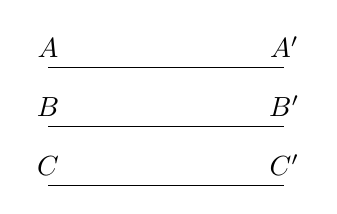
\begin{tikzpicture}[scale=0.75]
                              % Line for A--A'
                              \draw (0,0) -- (4,0);
                              \node[above]  at (0,0)   {$A$};
                              \node[above] at (4,0)   {$A'$};
                            
                              % Line for B--B'
                              \draw (0,-1) -- (4,-1);
                              \node[above]  at (0,-1)  {$B$};
                              \node[above] at (4,-1)  {$B'$};
                            
                              % Line for C--C'
                              \draw (0,-2) -- (4,-2);
                              \node[above]  at (0,-2)  {$C$};
                              \node[above] at (4,-2)  {$C'$};
                            \end{tikzpicture}
                        \end{center}
                        
                        \vspace{1em}
    
                        From the line AA', let the segment AE be subtracted:
    
                        \begin{center}
                            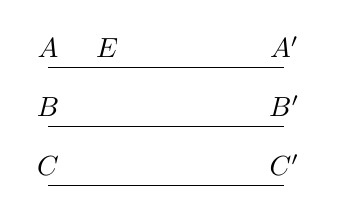
\begin{tikzpicture}[scale=0.75]
                              % A--E--A'
                              \draw (0,0) -- (4,0);
                              \node[above]  at (0,0)   {$A$};
                              \node[above] at (1,0)   {$E$};  % Place E somewhere between A and A'
                              \node[above] at (4,0)   {$A'$};
                            
                              % B--B'
                              \draw (0,-1) -- (4,-1);
                              \node[above]  at (0,-1)  {$B$};
                              \node[above] at (4,-1)  {$B'$};
                            
                              % C--C'
                              \draw (0,-2) -- (4,-2);
                              \node[above]  at (0,-2)  {$C$};
                              \node[above] at (4,-2)  {$C'$};
                            \end{tikzpicture}
                        \end{center}
                        
                        \vspace{1em}
    
                        and the segment CD added to the line CC', so that the whole line DCC' exceeds the line EA' by the segment CD and the segment CF; thus it exceeds the line BB' by the segment CD.
    
                        \begin{center}
                            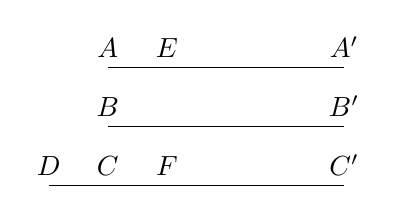
\begin{tikzpicture}[scale=0.75]
                              % A--E--A'
                              \draw (0,0) -- (4,0);
                              \node[above]  at (0,0)   {$A$};
                              \node[above] at (1,0)   {$E$};
                              \node[above] at (4,0)   {$A'$};
                            
                              % B--B'
                              \draw (0,-1) -- (4,-1);
                              \node[above]  at (0,-1)  {$B$};
                              \node[above] at (4,-1)  {$B'$};
                            
                              % D--C--F--C'
                              \draw (-1,-2) -- (4,-2);
                              \node[above]  at (-1,-2)  {$D$};
                              % Choose positions for C and F
                              \node[above] at (0,-2)  {$C$}; 
                              \node[above] at (1,-2)  {$F$};
                              \node[above] at (4,-2)  {$C'$};
                            \end{tikzpicture}
                        \end{center}
                        
                    \end{example}

\newpage

            \subsection{Two Kinds of Justice}

                \begin{definition}
                    \textbf{Distributive Justice} (Geometrical Proportion)
                    \begin{itemize}
                      \item Involves \textit{unequal} people (e.g., differing in merit) who should receive \textit{unequal} shares in proportion to their respective deserts.
                      \item Formula: $A : B = C : D$.
                    \end{itemize}
                \end{definition}

                \begin{definition}
                    \textbf{Rectificatory Justice} (Arithmetical Proportion)
                    \begin{itemize}
                      \item Involves \textit{equal persons} under the law who must be restored to a fair baseline when an injustice has occurred.
                      \item The judge ``corrects'' or ``rectifies'' by \textbf{subtracting} from the wrongdoer's gain and \textbf{adding} to the victim's loss.
                    \end{itemize}
                \end{definition}

                \subsubsection{Loss and Gain (revisited)}

                    \begin{itemize}
                      \item \textbf{Derivation}: The ideas of ``loss'' and ``gain'' come from \textit{voluntary exchange}, where one typically does not want to end up with less value (loss) or more than one's due (gain).
                      \item \textbf{Balance}: In just exchanges, each party ends with the value equivalent to what they began with, or at least with an agreed-upon equivalence of goods, services, or money.
                    \end{itemize}

            \subsection{Transactions}

                Aristotle divides transactions into:
                \begin{enumerate}
                  \item \textbf{Involuntary transactions}
                    \begin{itemize}
                      \item Examples: theft, assault, homicide, fraud, etc.
                      \item These necessitate the intervention of a judge or legal remedy to \textit{correct} (rectify) the imbalance.
                    \end{itemize}
                  \item \textbf{Voluntary transactions}
                    \begin{itemize}
                      \item Examples: commercial exchanges, renting, hiring, etc., where both parties consent.
                      \item These transactions \textit{can} still lead to disputes about ``gain'' and ``loss'' if the agreement is not honored or if one party defrauds the other.
                    \end{itemize}
                \end{enumerate}

                \subsubsection{Reciprocity}

                    Some philosophers (like the Pythagoreans) held that \textbf{reciprocity} (\emph{an eye for an eye}) is justice in an unqualified sense. However, Aristotle notes that strict reciprocity (literal tit-for-tat) does not accurately capture \textit{distributive} or \textit{rectificatory} justice, especially in cases where the parties' status is not the same (e.g., a citizen striking a magistrate might be punished more severely than if the roles were reversed).

                \subsubsection{Proportionate Reciprocation}\label{L1.2:Proportionate_Reciprocation}
                
                    Aristotle explains that in \textit{voluntary exchanges}, there is a form of justice he calls \textbf{``reciprocity in accordance with proportion.''} It is not mere equality of retaliation or transaction, but a reciprocal balance that accounts for the relative value of goods or services:
                    
                    \begin{quote}
                    If \textbf{A} is a builder and \textbf{B} is a shoemaker, and we want to exchange a house for shoes, the two must be \textit{commensurable} in a certain proportion so that the exchange is fair.
                    \end{quote}

        \section{A Third Kind of Justice}

            In addition to \textbf{distributive} and \textbf{rectificatory} justice, Aristotle explores a \textbf{third} concept often referred to as:
            \begin{quote}
            \[
            \text{\textit{antipeponthos kat' analogían}}
            \]
            \[
            \text{reciprocity in accordance with proportion.}
            \]
            \end{quote}

            This describes a kind of \textbf{proportional reciprocity} that arises especially in \textit{economic exchanges}, serving as the glue that holds a society together by rewarding good with good and returning bad with bad---yet doing so in proportion to the relative values or severity involved.

                \subsubsection{Proportionate Reciprocation}

                    When people engage in market exchanges, they must equate different goods in order to trade. Aristotle highlights:
                    \begin{itemize}
                      \item \textbf{A} (the builder)
                      \item \textbf{C} (a house)
                      \item \textbf{B} (the shoemaker)
                      \item \textbf{D} (shoes)
                    \end{itemize}

                    A fair exchange occurs when \textbf{A} receives from \textbf{B} a quantity of goods (shoes) that is proportionate in value to what \textbf{A} gives (a house). If one person's goods are inherently more valuable, the exchange ratio must reflect that.

            \subsection{Measure (The Role of Money)}

                Because houses, shoes, and other goods are not easily compared, society uses \textbf{money} as a conventional measure:
                \begin{enumerate}
                  \item Money acts as a \textbf{mean}, making goods and services \textbf{commensurable}.
                  \item It provides a universal measure of value so that we can compare ``how many shoes equal one house.''
                \end{enumerate}
                
                Aristotle derives the Greek word for money, \emph{nomisma}, from \textit{nomos} (law or convention), to emphasize that money's value is established by collective agreement. Without money, trade would rely on barter, which complicates finding fair ratios (how many shoes per house?).

                \subsubsection{Proportional Reciprocity in Practice}

                    It is not that two doctors exchange services, but rather a farmer and a doctor, or a builder and a shoemaker. Because these parties produce different and \textit{unequal} things, there must be a standardized method (money) to equate and balance their transactions. This fosters \textbf{social cohesion}: people exchange goods or services in proportion to their value, keeping relationships functional and the city unified.

        \section*{L1.2 -- Conclusions}

            Aristotle's discussion in Book V of the \textit{Nicomachean Ethics} reveals how \textbf{justice} can be understood in several overlapping senses:
            \begin{enumerate}
              \item \textbf{Distributive justice} deals with proportional allocations to \textbf{unequal} persons, according to their merit (geometrical proportion).
              \item \textbf{Rectificatory justice} addresses the correction of wrongs through \textbf{arithmetical} proportion, treating the parties as equals before the law, subtracting from the wrongdoer's excess and compensating the victim's loss.
              \item \textbf{Proportionate reciprocity} (sometimes taken as a \textbf{third} kind of justice) emphasizes fair exchange in economic or social transactions, achieved through a \textbf{proportional} equality rather than mere equality. Money becomes a key instrument for measuring and making commensurable the goods or services exchanged.
            \end{enumerate}
            
            \begin{remark}
                In \textbf{distributive} justice, differences in people's status or merit lead to \textbf{unequal} allocations that are still fair because they are \textit{proportionate}. In \textbf{rectificatory} justice, the parties are treated as \textbf{equals} in the sense that the law imposes a correction for the wrongdoing. In \textbf{exchange}, people's different products or services must be brought into a \textbf{proportionate} equality so that trade can occur fairly.
            \end{remark}

            \begin{remark}[Why we use mathematics in \ref{L1.2:Proportionate_Reciprocation}]
                From the greek ``\textit{mathēmatikē}'', from the base of ``\textit{manthanein}'', to learn. It is simply more logical to argue via the use of math, as it allows us to uncover and argue for something that is already known.
            \end{remark}
            
            Aristotle's overarching conclusion is that although all three share something in common---namely, the idea of \textbf{balance} or \textbf{mean}---they apply in different realms (distribution of public goods, correction of private harms, and exchange of goods/services). Where \textbf{distributive justice} and \textbf{rectificatory justice} ``rectify'' imbalances by either awarding shares in proportion to merit or compensating losses, \textbf{proportionate reciprocity} emphasizes mutual benefit and the cohesive power of fair trade in the city.
            
            Thus, differences are recognized---merit, wrongdoing, product value---but justice seeks to bring them into a \textbf{measured} or \textbf{proportional} equilibrium, preserving harmony and fairness in social life.


    \chapter[Just Price and Quantities of Labour]{Thomas Aquinas \\[0.6cm] \textit{Just Price and Quantities of Labour}}

        \section{\textit{Summa Theologiae}}

    \begin{remark}
        Thomas Aquinas’s discussion of \textit{just price} and related issues in buying and selling draws heavily on Aristotle’s works, most notably \textit{Politics} (Book I) and \textit{Nicomachean Ethics} (Book V). It also engages with classical examples provided by Cicero (e.g., \textit{De Officiis}) and relies on Roman law regarding contracts and fairness (\textit{Codex Iustinianus}).
    \end{remark}

    \subsection{Question 77: On cheating in buying and selling}

        \subsubsection{Article 3. Whether the seller is bound to state the defects of the thing sold}

            \begin{quote}
                Suppose, for example, a time of dearth and famine at Rhodes, with provisions at fabulous prices; and suppose that an honest man has imported a large cargo of grain from Alexandria and that to his certain knowledge also several other importers have set sail from Alexandria, and that on the voyage he has sighted their vessels laden with grain and bound for Rhodes; is he to report the fact to the Rhodians or is he to keep his own counsel and sell his own stock at the highest market price?
            
                (Cicero, \textit{De Officiis}, Book 3.50)
            \end{quote}
    
            \begin{quote}
                [...] it is not in accord with Nature that anyone should take advantage of his neighbour’s ignorance.
            
                (Cicero, \textit{De Officiis}, Book 3.72)
            \end{quote}
    
            Aquinas distinguishes between hiding an actual, present defect in goods versus simply withholding information about future events. A defect in a thing lessens its value \emph{in the present}, while in the Rhodes example the coming arrival of additional grain will lessen the price \emph{in the future}. Since future circumstances are by definition uncertain to the buyer, Aquinas holds that the seller who sells at the current market price does not commit an injustice merely by not revealing the future influx of grain. He does acknowledge that revealing such information or voluntarily lowering the price would be more virtuous, but it is not strictly required by justice.
    
            \begin{quote}
                \textit{Ad quartum dicendum quod vitium rei facit rem in praesenti esse minoris valoris quam videatur, sed in casu praemisso, in futurum res expectatur esse minoris valoris per superventum negotiatorum, qui ab ementibus ignoratur. Unde venditor qui vendit rem secundum pretium quod invenit, non videtur contra iustitiam facere si quod futurum est non exponat. Si tamen exponeret, vel de pretio subtraheret, abundantioris esset virtutis, quamvis ad hoc non videatur teneri ex iustitiae debito.}
            \end{quote}
    
            \begin{remark}
            Aquinas concludes that such a situation is \emph{not} a fraud in the strict sense but rather a change in circumstance (present vs.\ future). In other words, if the item truly has a defect in the here and now, the seller is obliged to disclose it; if the expected lowering of the price is only in the future, one is not strictly obligated to mention it.
            \end{remark}
    
            Aquinas also draws on Aristotle’s principle that transactions \emph{ought} to observe an “equality of thing and thing.” Yet, in practical realities, exceptions may occur without constituting injustice.

        \subsubsection{Article 4. Whether, in trading, it is licit to sell a thing at a higher price than what was paid for it}

            \begin{quote}
                A tradesman is one whose business consists in the exchange of things. According to the Philosopher (Polit. i, 3), exchange of things is twofold: one, natural as it were, and necessary, whereby one commodity is exchanged for another, or money taken in exchange for a commodity, in order to satisfy the needs of life. Such like trading, properly speaking, does not belong to tradesmen, but rather to housekeepers or civil servants who have to provide the household or the state with the necessaries of life. 
            
                The other kind of exchange is either that of money for money, or of any commodity for money, not on account of the necessities of life, but for profit, and this kind of exchange, properly speaking, regards tradesmen, according to the Philosopher (Polit. i, 3). The former kind of exchange is commendable because it supplies a natural need: but the latter is justly deserving of blame, because, considered in itself, it satisfies the greed for gain, which knows no limit and tends to infinity.
            \end{quote}

            Aquinas remarks that trading for profit \emph{by itself} does not necessarily entail sinfulness, provided the intention is just. It becomes permissible if one’s ultimate goal is, for example, the upkeep of one’s household or the relief of the poor, rather than an endless accumulation of wealth. In such cases, a markup can be seen as “\textit{stipendium laboris},” i.e., compensation for labor, transport, or risk.

            \begin{quote}
                Hence trading, considered in itself, has a certain debasement attaching thereto, in so far as, by its very nature, it does not imply a virtuous or necessary end. Nevertheless gain which is the end of trading, though not implying, by its nature, anything virtuous or necessary, does not, in itself, connote anything sinful or contrary to virtue: wherefore nothing prevents gain from being directed to some necessary or even virtuous end, and thus trading becomes licit. [...] For if he sells at a higher price something that has changed for the better, he would seem to receive the reward of his labour.
            \end{quote}

            The key point is that if the item truly \emph{increases in value}—either because of the labor expended in improving it, or because of the costs (danger, transportation, etc.) involved—charging a higher price is legitimate and does not violate justice.

    \subsection{Question 61: The parts of Justice}

        Aquinas notes that Aristotle, in \textit{Nicomachean Ethics} Book V, distinguishes two basic forms of justice:
        \begin{enumerate}
            \item \textbf{Distributive justice}, whose mean is determined by \emph{geometrical proportion}. Those who are more “worthy” (e.g., possessing higher rank, ability, or contribution to the common good) receive proportionally more from the common stock.
            \item \textbf{Commutative (or Corrective) justice}, whose mean is determined by \emph{arithmetical proportion}. This applies to voluntary exchanges (like buying and selling) or involuntary exchanges (like theft or violence). Here we do not weigh personal status but rather strictly ensure that each party receives or restores an amount equal to what was lost or gained.
        \end{enumerate}

        \begin{quote}
            The Philosopher says (Ethic. v, 3,4) that the mean in distributive justice is observed according to ``geometrical proportion,'' whereas in commutative justice it follows “arithmetical proportion.” [...]
            
            On the other hand, in commutations something is paid to an individual on account of something of his that has been received [...] Hence it is necessary to equalize thing with thing, so that the one person should pay back to the other just so much as he has become richer out of that which belonged to the other. [...]
        \end{quote}

        \begin{remark}
            Aquinas \emph{collapses} many possible distinctions of exchange (including punitive “contrapassum”) into commutative justice. This allows a judge or an authority, if needed, to impose restitution or compensation and thereby restore equality.
        \end{remark}

        He also explains the notion of \emph{reciprocity} (\textit{contrapassum}), i.e.\ returning harm for harm, or restitution for what was taken:
        
        \begin{quote}
            Reciprocity [\textit{contrapassum}] denotes equal passion repaid for previous action; and the expression applies most properly to injurious passions and actions, whereby a man harms the person of his neighbor; for instance if a man strike, that he be struck back. [...] And since also to take away what belongs to another is to do an unjust thing, it follows that secondly reciprocity consists in this also, that whosoever causes loss to another, should suffer loss in his belongings, [...]. 
        \end{quote}
        
        Yet perfect equality is not always straightforward: striking a mere citizen versus striking a prince, for example, might receive different punishments to maintain the proportional or corrective “mean.” Likewise, theft or fraud in property may be punished by returning more than the stolen value, taking into account the harm to the wider community.

    \subsection*{Back to Question 77: On cheating in buying and selling}

        \subsubsection{Article 1. Whether it is licit to sell a thing for more than its value}

            Aquinas clarifies that employing deceit is always sinful. But absent deceit, there are two main considerations:
            
            \begin{enumerate}
                \item \emph{Buying and selling considered in themselves}. In principle, exchange is for the mutual advantage of both parties. This requires an equality of “thing and thing” and the avoidance of exploitation. Money was introduced exactly to measure this equivalence. If the \emph{price} unreasonably exceeds the \emph{thing’s value} (or vice versa), it violates commutative justice.
            
                \item \emph{Buying and selling considered in relation to special circumstances}. For instance, if the seller will incur a particular \emph{loss} or bears certain costs or risks, the “just price” can rightly be higher. Thus Aquinas allows selling at a higher price if that higher price genuinely reflects additional expenses, risks, or the utility the buyer personally attributes to the good.
            \end{enumerate}
            
            He also references how different legal or moral systems might respond. \emph{Human law} may tolerate certain lesser injustices and only punish more egregious ones (e.g., cases involving an overcharge greater than half the thing’s value, referencing Roman law on \textit{laesio enormis}). \emph{Divine law}, on the other hand, leaves nothing unpunished that is contrary to virtue. 

            \begin{quote}
                Accordingly, if without employing deceit the seller sells his goods overvaluing them (\textit{rem suam supervendat}), or the buyer obtain them for less, the law looks upon this as licit, and provides no punishment for so doing, unless the excess be too great, because then even human law demands restitution to be made [...]. 
                
                On the other hand, the Divine law leaves nothing unpunished that is contrary to virtue. [...] I add this condition, because the just price of things (\textit{iustum pretium rerum}) is not precisely determined (\textit{non est punctualiter determinatum}), but consists in a kind of estimate (\textit{in quadam aestimatione consistit}), so that a slight addition or subtraction would not seem to destroy the equality of justice.
            \end{quote}
            
            In other words, prices often involve an \emph{estimate} (because the “exact” value of a thing can be hard to establish). So minor deviations need not be considered injustice, but significant deviations may require restitution.

\section{Commentary on Aristotle's \textit{Nicomachean Ethics}}

    Aquinas’s \textit{Commentary on the Nicomachean Ethics} further discusses how just exchange depends on proportional equivalences:
    
    \begin{quote}
        971. Next […], he [Aristotle] explains in what matter and manner the statement is true that reciprocation is justice. He discusses this point from three aspects. First [III, A] he shows that there must be reciprocation in exchanges according to proportionality. Then […], he explains the form of this proportionality. Last [Lect. 9; C], at “Therefore all etc.” (B. 1133 a 18), he shows how such a form can be observed. […] He says that in dealings of exchange it is true that justice is of such a nature that it includes reciprocation not according to equality but according to proportionality.
    \end{quote}
    
    \begin{quote}
        972. It seems this is contrary to what was said before (950), that in commutative justice the mean is taken not according to geometrical proportionality, which consists in an equality of proportion, but according to arithmetic proportionality, which consists in a quantitative equality. We must say that, in regard to commutative justice there should always be an equality of thing to thing, not, however, of action and passion, which implies corresponding requital. But in this, proportionality must be employed in order to bring about an equality of things because the work of one craftsman is of more value than the work of another, e.g., the building of a house than the production of a penknife. Hence, if the builder exchanged his work for the work of the cutler, there would not be equality of thing, given and taken, i.e., of house and penknife.
    \end{quote}

    Here, Aquinas’s point (following Aristotle) is that \emph{some} form of proportional balancing is needed so that, for example, the combined labor or value put into \emph{many} sandals might properly match the labor or value of building a \emph{house}. Strict one-for-one exchange of different goods could be obviously unfair.

    \begin{quote}
        980. Next […], he shows how exchange takes place according to the preceding commensuration. Although a house is worth more than a sandal, nevertheless, a number of sandals are equal in value to one house or the food required for one man during a long period. [...] If this is not observed, there will be no exchange of things and men will not share their goods with one another.
    \end{quote}
    
    \begin{quote}
        983. Then […], he shows how just reciprocation takes place in exchanges according to the preceding commensuration. [...] He says first that the norm measuring all things by need according to nature and by currency according to human convention will then become reciprocation when everything will be equated in the way just mentioned.
    \end{quote}
    
    Aquinas explains Aristotle’s use of a “proportional figure with diagonals”—the well-known schematic in Book V of the \textit{Nicomachean Ethics}—to illustrate how different trades and values must be matched in some ratio. If the builder invests more labor or expense, that difference should be compensated by a correspondingly larger quantity of goods from the other party.

    \begin{quote}
        Thus, when exchange of things (\textit{commutatio rerum}) takes place, the articles to be exchanged (\textit{res commutandas}) ought to be arranged in a proportional figure with diagonals, as was stated previously (957). If this was not done, one extreme would have both excesses (\textit{superabundantias});
    
        if a farmer gave a bushel of wheat for a sandal, he would have an excess of labour in his product (\textit{superabundantiam laboris in opere}) and would have also an excess of presents (\textit{superabundantiam doni}) because he would be giving more than he would receive. But when all have what is theirs, they are in this way equal and do business with one another because the equality previously mentioned is possible for them.
    \end{quote}

\section*{Additional Context and Observations}

    \begin{remark}[Roman Law and the “Just Price”]
        Aquinas’s notion of \emph{just price} was influenced by Roman legal principles, such as those found in the \textit{Codex Iustinianus}. One doctrine, \textit{laesio enormis}, allowed a contract to be rescinded if it was made at less than half of the fair market value. Aquinas often reconciles such legal norms with moral theology: human law tolerates smaller deviations but punishes larger ones.
    \end{remark}

    \begin{remark}[Moral vs. Legal Dimensions]
        Aquinas’s distinction between the requirements of \emph{human law} and \emph{divine law} underscores that, from the standpoint of perfect virtue, even smaller injustices in exchange can be blameworthy. However, civil law ordinarily penalizes only the more severe cases so that social order remains manageable among “many lacking in virtue.”
    \end{remark}

    \begin{remark}[Natural vs. Unnatural Exchange (Aristotle’s Framework)]
        Following Aristotle, Aquinas differentiates between (a) \emph{natural exchange}, which serves to provide for genuine needs (e.g., household provisioning) and is seen as ethically commendable, and (b) \emph{unnatural or artificial exchange}, which solely pursues profit or speculation. This latter is neither intrinsically sinful nor virtuous but can become morally questionable when it stems from greed or exploits others.
    \end{remark}

    \begin{remark}[Labour, Risk, and Transportation]
        Aquinas consistently holds that a higher selling price may be justified when it compensates for improvements, labour, transport costs, or risk borne by the merchant. Thus, “buying low and selling high” is not automatically unjust; it depends on whether the markup is proportionate to real added value or costs.
    \end{remark}

    \begin{remark}[Practical Applicability]
        Although Aquinas lived in a medieval context (13th century), his arguments about honesty in trade, transparency of defects, and fairness in pricing remain influential in discussions of market ethics, consumer protection, and economic justice today.
    \end{remark}

        \subsubsection{Final considerations}

    \noindent In summary, Aquinas’s teaching on just price centres on the principle that transactions must preserve a certain equality, measured not only by the intrinsic worth of the item but also by factors such as labour input, risk undertaken, and legitimate need of both parties. While human law may choose to tolerate minor deviations from perfect equity, moral theology requires that all intentional distortion or fraud be avoided. Exchanges should, as far as possible, reflect a mutual benefit and fair equivalence between what is given and what is received—a principle that finds its roots in both Aristotelian philosophy and the broader Christian moral tradition.


    \chapter[Survival and the state of nature]{Thomas Hobbes \\[0.6cm] \textit{Survival and the state of nature}}

        \vspace{-0.5cm}

    \subsection*{Historical Context}

        \begin{itemize}
          \item \textbf{Protestant Reformation (1517)}
            \begin{itemize}
              \item Initiated by Martin Luther, leading to significant religious and political upheaval in Europe.
              \item Contributed to the fragmentation of the Catholic Church and fueled inter-state and intra-state conflicts.
            \end{itemize}
        
          \item \textbf{European Religious Wars (16th--17th centuries and beyond)}
            \begin{itemize}
              \item Culmination of tensions between Protestants and Catholics, as well as between different Protestant factions.
              \item These conflicts ravaged many European regions, fostering an environment of mistrust, instability, and the need for strong governance.
            \end{itemize}
        
          \item \textbf{Scientific Revolution: Galileo (1564--1642), Descartes (1596--1650)}
            \begin{itemize}
              \item A shift toward empiricism and rational inquiry.
              \item Galileo’s emphasis on observation and mathematics, and Descartes’ focus on methodic doubt and the primacy of reason, challenged traditional Scholastic frameworks in philosophy and natural science.
            \end{itemize}
        
          \item \textbf{English Civil War (1642--1651)}
            \begin{itemize}
              \item Fought between Royalists (supporters of King Charles I) and Parliamentarians (supporters of parliamentary power).
              \item Thomas Hobbes lived through this period of turmoil. His experiences informed his conviction that strong central authority is necessary to prevent civil strife.
            \end{itemize}
        \end{itemize}

        These historical factors deeply influenced Hobbes’s thinking. The \textit{Protestant Reformation} and the ensuing religious wars showed him how divergent beliefs can destabilize entire societies, while the \textit{Scientific Revolution} shaped his mechanical, materialist approach to human cognition and social organization. The immediate political unrest of the \textit{English Civil War} offered him a firsthand example of the dangers of insufficiently centralized power.

\section{\textit{Leviathan} (1651)}

    Thomas Hobbes’s \textit{Leviathan} is one of the foundational texts of modern political philosophy. Published amidst the chaos of the English Civil War, it offers a rigorous defense of absolute sovereignty as a means to ensure peace and security. Before discussing the notion of the commonwealth, Hobbes establishes the philosophical basis of his approach by explaining his conception of sense, imagination, and the motions that drive human passions.

        \subsubsection{The Origin of Our Thoughts}

            \begin{quote}
                Concerning the thoughts of man, I will consider them first singly, and afterwards in train or dependence upon one another. Singly, they are every one a representation or appearance of some quality, or other accident of a body without us … The original of them all is that which we call SENSE … The rest are derived from that original.
            \end{quote}

            Hobbes begins by describing \textbf{thought} and \textbf{consciousness} as fundamentally connected to \textbf{sense experience}. For him, all cognition---every idea, concept, or thought---can be traced back to an external object pressing upon our sensory organs. This “pressing” or “motion” triggers internal changes that we register as sense impressions.

            \begin{remark}
                \begin{itemize}[leftmargin=*]
                    \item There is no content in the mind that did not first originate in sense (a direct challenge to the idea of innate knowledge).
                    \item Thought builds upon and rearranges these original sensory inputs over time.
                \end{itemize}
            \end{remark}

        \subsubsection{The Cause of Sense}

            \begin{quote}
            The cause of sense is the external body, or object, which presseth the organ proper to each sense … which pressure … continued inwards to the brain and heart, causeth there a resistance, or counter-pressure … which endeavour, because outward, seemeth to be some matter without.
            \end{quote}

            For Hobbes, \textbf{sense} arises through a mechanical process: external objects literally press upon our sense organs (directly for taste and touch, or indirectly for vision and hearing), causing a chain reaction of motions. Hobbes is adopting the nascent mechanical philosophy of his era, influenced by thinkers like Galileo, who emphasized that \textbf{all observable phenomena} (including perception) can be explained in terms of matter and motion.

        \subsubsection{Several Motions of the Matter}

            \begin{quote}
                All which qualities called sensible are in the object that causeth them but so many several motions of the matter … Neither in us that are pressed are they anything else but diverse motions … But their appearance to us is fancy, the same waking that dreaming.
            \end{quote}
            
            Here, Hobbes extends this mechanical explanation to clarify that what we perceive as “heat,” “cold,” “color,” or “sound” is actually the effect of \textit{various motions} in objects interacting with our organs. The “qualities” we perceive---like color---are not identical to anything literally colored existing outside us, but rather the result of our nervous system’s interpretation of motion.

In modern philosophy, this distinction is sometimes referred to as the difference between:
\begin{itemize}
  \item \textbf{Primary qualities} (e.g., extension, motion) which inhere in objects themselves.
  \item \textbf{Secondary qualities} (e.g., color, taste, sound) which are the mind’s interpretation of those motions.
\end{itemize}

\section*{The Object Is One Thing, the Image Is Another}

\begin{quote}
\textit{“... yet still the object is one thing, the image or fancy is another. So that sense in all cases is nothing else but original fancy caused … by the motion of external things upon our eyes, ears, and other organs ...”}
\end{quote}

This underlines Hobbes’s \textbf{representational} theory of perception: there is always a distinction between the external thing and the mental image or representation we have of it. He emphasizes that the process by which we see or hear something resembles the effect of physically pressing upon the relevant sense organ.

\section*{Chapter 1 -- \textit{Of Sense}}

\begin{remark}
\begin{itemize}
  \item The origin of thought is \textbf{sense}.
  \item The origin of sense is an \textbf{impression} (motion) from an external object.
  \item \textbf{Sense} is an \textbf{appearance} that does not coincide exactly with the object that caused it.
\end{itemize}
\end{remark}

\section*{Opposition to Scholasticism}

\begin{quote}
\textit{“But the philosophy schools, through all the universities of Christendom, grounded upon certain texts of Aristotle, teach another doctrine … they say, for the cause of vision, that the thing seen sendeth forth on every side a visible species … I say not this, as disapproving the use of universities: but … the frequency of insignificant speech is one.”}
\end{quote}

\subsubsection*{Hobbes vs. Aristotelian-Scholastic Philosophy}
Hobbes rejects the \textbf{Scholastic} notion of “species” or “forms” emanating from objects. According to the Aristotelian tradition, a “visible species” travels to our eyes, or an “audible species” reaches our ears. Hobbes sees these explanations as outdated and unnecessarily obscure, preferring instead a mechanistic, matter-in-motion account of perception.

\section*{Digression: Aristotle}

Hobbes draws heavily on certain parts of \textbf{Aristotle’s} thought (particularly regarding motion and potentiality), but discards other aspects (like species forms). Still, Aristotle’s concepts of \textit{dynamis} (potential) and \textit{energeia} (actualization) remain instructive:

\begin{remark}
There is not just one pressure or force, but two capacities or dispositions:
\begin{itemize}
  \item \textbf{Dynamis}: The potential or capacity (movement, tension)
  \item The meeting of two dispositions leads to \textbf{energeia} (the actualization)
\end{itemize}
\end{remark}

\subsubsection*{Aesthetics (Aisthesis)}
From the viewpoint of sensing (\textit{aisthesis}):
\begin{itemize}
  \item \textbf{Two dynamis}:
  \begin{enumerate}
    \item The table has the capacity or disposition to be seen.
    \item I have the capacity or disposition to see.
  \end{enumerate}
  \item \textbf{Energeia}:
    \begin{itemize}
      \item When these capacities meet, I \textit{actually} see the table, and the table \textit{is seen}.
    \end{itemize}
\end{itemize}

\subsubsection*{Technique (Techn\'e)}
From the viewpoint of \textit{techn\'e} (technique, or purposeful use):
\begin{itemize}
  \item \textbf{Two dynamis}:
  \begin{enumerate}
    \item The table has the capacity to be used (it is “ready” for use).
    \item I have the capacity to use it.
  \end{enumerate}
  \item \textbf{Energeia}:
    \begin{itemize}
      \item I \textit{use} the table, and the table \textit{is used} by me.
    \end{itemize}
\end{itemize}

In \textbf{Scholastic terms} (Aquinas), these are “potentia” and “actus.” In \textbf{Hobbesian} terms, power is simply \textit{motion} in matter. The important distinction is that Hobbes explains both sense and action via \textit{mechanical} cause and effect.

\section*{Chapter 2 -- \textit{Of Imagination}}

\begin{quote}
\textit{“That when a thing lies still … it will lie still for ever … is a truth that no man doubts of. But that when a thing is in motion, it will eternally be in motion, unless somewhat else stay it … is not so easily assented to.”}
\end{quote}

Hobbes explicitly references \textbf{Galileo’s} principle of inertia (bodies in motion continue in motion unless acted upon). He extends this to mental phenomena, arguing that \textbf{imagination} is simply the “decaying sense” left over after an original sensation has passed.

\section*{Chapter 6 -- \textit{Of the Interior Beginnings of Voluntary Motions, commonly called Passions}}

\subsubsection*{Vital and Animal Motion}

\begin{quote}
\textit{“There be in animals two sorts of motions peculiar to them: One called vital … the other is animal motion, otherwise called voluntary motion … that sense is motion … fancy is but the relics of the same motion … has been already said in the first and second chapters.”}
\end{quote}

\begin{itemize}
  \item \textbf{Vital motions}: Automatic processes (circulation, respiration, digestion) that do not require conscious thought.
  \item \textbf{Animal/Voluntary motions}: Actions we deliberately choose (walking, speaking) based on images or ideas in the mind.
\end{itemize}

\subsubsection*{Small Beginnings of Motion}

\begin{quote}
\textit{“These small beginnings of motion within the body of man, before they appear in walking … are commonly called endeavour.”}
\end{quote}

Hobbes introduces “\textbf{endeavour}” (\textit{conatus}): the minute, preconscious stirrings that set us on a particular path to act. Every deliberate act is preceded by this subtle motion in the mind and body.

\begin{itemize}
  \item \textbf{Desire} (or appetite) is endeavour \textbf{toward} something.
  \item \textbf{Aversion} is endeavour \textbf{away} from something.
\end{itemize}

\section*{Chapter 9 -- \textit{Of the Difference of Manners}}

\subsubsection*{Felicity Is Not Satisfaction}

\begin{quote}
\textit{“For there is no such finis ultimus (utmost aim) nor summum bonum (greatest good) … Felicity is a continual progress of the desire from one object to another, the attaining of the former being still but the way to the latter.”}
\end{quote}

Contrary to the ancient and medieval idea of a highest good or final end (e.g., \textit{eudaimonia} or \textit{beatitudo}), Hobbes argues that \textbf{human life} is characterized by \textbf{endless striving}. People are driven to seek power, comfort, and security continually; there is no final stopping point of perfect contentment.

\subsubsection*{A Restless Desire of Power After Power}

\begin{quote}
\textit{“... a perpetual and restless desire of power after power, that ceaseth only in death.”}
\end{quote}

This emphasis on \textbf{power} clarifies one of Hobbes’s most famous theses: humans are consistently compelled to increase their power---not necessarily out of boundless ambition, but often out of fear. Since one can never be sure that present power is sufficient for future security, individuals feel driven to acquire more.

\section*{Chapter 13 -- \textit{Of the Natural Condition of Mankind as concerning their Felicity and Misery}}

\subsubsection*{Diffidence of One Another}

\begin{quote}
\textit{“... if one plant, sow, build, or possess a convenient seat, others may probably be expected to come ... to dispossess and deprive him, not only of the fruit of his labour, but also of his life or liberty.”}
\end{quote}

In the \textbf{State of Nature}, Hobbes sees \textit{diffidence}---basic mistrust---of one another as inevitable. Since no central authority holds us in check, we are perpetually at risk of predation by others.

\subsubsection*{Anticipation}

\begin{quote}
\textit{“And from this diffidence of one another, there is no way for any man to secure himself so reasonable as anticipation ...”}
\end{quote}

Hobbes famously argues that a rational person in the state of nature will often strike first. Fear compels us to \textit{anticipate} aggression by others, leading us to preemptively attack. This dynamic feeds a cycle of insecurity and violence.

\subsubsection*{War Against All}

\begin{quote}
\textit{“... during the time men live without a common power to keep them all in awe, they are in that condition which is called war; and such a war as is of every man against every man.”}
\end{quote}

This condition is not limited to open combat but is any period during which there is a \textit{known disposition} to fight. Peace, by contrast, is the period during which mutual assurance exists under a power capable of enforcing it.

\section*{\textit{Homo Homini Lupus}}

This famous Latin phrase---“man is a wolf to man”---captures Hobbes’s view that humans, left to their own devices in the state of nature, revert to predatory behavior. Hobbes did not coin the phrase himself (it has roots in Plautus), but he popularized its application to early modern political thought.

\subsubsection*{No Place for Industry}

\begin{quote}
\textit{“In such condition there is no place for industry … and which is worst of all, continual fear, and danger of violent death; and the life of man, solitary, poor, nasty, brutish, and short.”}
\end{quote}

Hobbes explains that in a perpetual state of war and insecurity, \textbf{cultural and economic life} cannot flourish. There can be no advanced agriculture, no trade, no arts, and no lasting human cooperation because all fruits of labor remain exposed to theft or destruction.

\subsubsection*{No Pleasure in Keeping Company}

\begin{quote}
\textit{“Again, men have no pleasure … in keeping company where there is no power able to overawe them all.”}
\end{quote}

The entire purpose of coming together in \textbf{civil society}---establishing a commonwealth---is precisely to avoid this mutual fear. While humans are not \textit{naturally} social in Hobbes’s view (rejecting Aristotle’s \textit{zoon politikon} thesis), their recognition of danger eventually compels them to form society.

\begin{remark}
\begin{itemize}
  \item A \textbf{human being} is neither a \textit{zoon politikon} (naturally political animal) nor an \textit{animal sociale} (a naturally sociable being).
  \item \textbf{In the state of nature}, human beings are antisocial and in constant fear of one another.
  \item \textbf{Paradoxically}, it is this mutual fear that drives individuals to form a civil society under a powerful sovereign who enforces peace.
\end{itemize}
\end{remark}

\section*{Conclusion and What Might Be Missing}

\subsection*{Toward the Social Contract}
Although these notes end with Hobbes’s description of the “war of all against all,” a further crucial step is Hobbes’s argument about how rational individuals \textbf{escape} the state of nature. In chapters that follow (especially Chapters 14--17 of \textit{Leviathan}), Hobbes outlines how people, motivated by fear of violence, willingly give up certain natural rights to a sovereign power in a \textbf{social contract}. This sovereign---represented as the “Leviathan”---possesses enough strength to enforce peace and cooperation.

\subsection*{Mechanistic Worldview and Politics}
One of Hobbes’s \textit{unique contributions} is applying the mechanical worldview (inspired by Galileo and Descartes) to \textbf{political} and \textbf{ethical} questions. He explains both mental processes (imagination, desire, aversion) and social relations (the state of nature, conflict, the institution of sovereignty) in terms of bodies in motion, pressing and resisting one another.

\subsection*{Key Themes Often Discussed Alongside Hobbes}
\begin{itemize}
  \item \textbf{Epistemology and Science}: Hobbes’s insistence that sense comes from matter in motion places him among the early pioneers of modern empiricism.
  \item \textbf{Materialism}: Hobbes famously argued that even mental phenomena could be explained physically, challenging dualist philosophies.
  \item \textbf{Absolutism vs. Individual Rights}: Hobbes’s proposed solution---absolute sovereignty---was controversial, especially among those defending constitutional limitations.
  \item \textbf{Continuing Influence}: Hobbes’s ideas on fear, power, and contract theory laid groundwork for later Enlightenment thinkers like John Locke (who diverged on many points) and Jean-Jacques Rousseau.
\end{itemize}

\section*{Final Remarks}
These expanded notes cover both Hobbes’s \textbf{philosophical method} (rooted in the mechanical account of sense and imagination) and his \textbf{political vision} (the necessity of a common power to avoid the misery of war). The \textbf{historical context} underscores how the upheavals of the Reformation, religious strife, and civil war shaped Hobbes’s central claim: only a powerful, unified authority can tame the otherwise fearful and violent human condition.

If you plan to delve deeper into \textit{Leviathan}, consider exploring:
\begin{itemize}
  \item Hobbes’s \textbf{laws of nature} and how they underpin the social contract.
  \item His notion of \textbf{sovereignty}---the “mortal god”---and how it relates to individual liberty.
  \item His critique of alternative political theories, including rival contract theorists and the \textbf{Aristotelian-Scholastic} tradition he found so lacking.
\end{itemize}

All these elements together form one of the most influential and enduring works of modern political philosophy.


    \chapter[Natural price and moral quantities]{Samuel Pufendorf \\[0.6cm] \textit{Natural price and moral quantities}}

    \chapter[Unsocial sociability and the tug of war]{Bernard Mandeville \\[0.6cm] Unsocial sociability and the tug of war}

    \chapter[Pleasure of exchange and progressive state]{Adam Smith \\[0.6cm] \textit{Pleasure of exchange and progressive state}}

    \chapter[Private property and communism]{Karl Marx \\[0.6cm] \textit{Private property and communism}}

    \chapter[Perfect competition and paradox of uncertainty]{Franck Knight\\[0.6cm] \textit{Perfect competition and the paradox of uncertainty}}

    \chapter[Crisis, uncertainty and animal spirits]{J.M. Keynes \\[0.6cm] \textit{Crisis, uncertainty and animal spirits}}

\part{Public Policy and Administration}

    \chapter{TBD}

\end{document}
